\documentclass[12pt]{article}

\author{Pablo Vargas Bermúdez}

\usepackage{minted}
\usepackage[margin=3cm]{geometry}
\usepackage{graphicx}
\usepackage{pdfpages}

\begin{document}
\pagestyle{empty}

\includepdf[pages=-]{Portada}

\section*{Planteamiento}

Programa hecho durante la clase donde se muestra información con
respecto a un listado de alumnos, Agregar un escucha donde la columna
seleccionada muestre en una etiqueta ubicada en el sur de la ventana
la información del registro seleccionado.

\section*{Código}

\subsection*{Clase Data}
\inputminted{Java}{Data.java}
\subsection*{Clase Gui}
\inputminted{Java}{Gui.java}
\subsection*{Clase de prueba}
\inputminted{Java}{Prueba.java}

\section*{Ejecución}

\begin{figure}[ht]
  \centering
  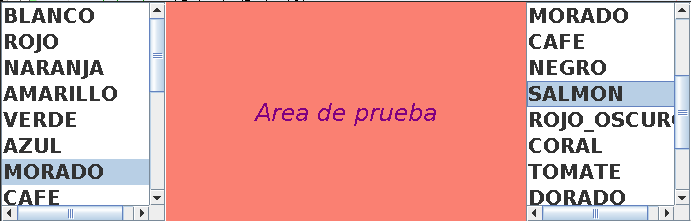
\includegraphics[width=\textwidth]{figures/run1.png}
  \caption{Primera prueba}
\end{figure}

\begin{figure}[ht]
  \centering
  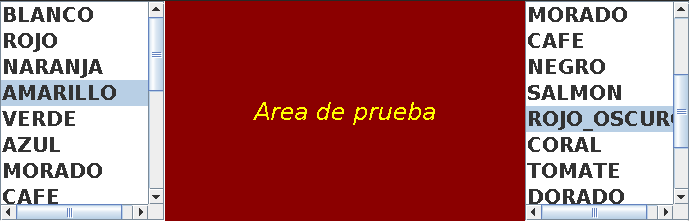
\includegraphics[width=\textwidth]{figures/run2.png}
  \caption{Segunda prueba}
\end{figure}

\end{document}
